% Overview of the information flow properties and applications:

% THIS IS A DUMP OF THE CONTENTS OF THE PAPER FROM 4-25-2016 -- update me with edits.

\chapter{Information Flow Analysis of Distributed Computing}


\section{Methods}

A model created for a distributed system must have sufficient information to create an accurate model. This information is difficult to obtain because of the circumstances many distributed systems run on. Without exact synchronization, an accurate global snapshot of the system cannot be taken. Instead of attempting to capture exact global snapshots, our approach relies on allowing an agent to reason about the state of the other agents in the system in order to allow that agent to construct a model which can then be distributed to other agents.


To do this we propose the following structure for the execution environment of the distributed system:
Each agent has some set logical atoms which it manipulates as its algorithms execute.
Each agent belongs to domain unique to that agent (agent $i$ is the only member of logical domain $D_i$)
No agent can directly access a logical atom outside of its domain.
The authenticity of any information transfer (Using modal operator $I_{i,j}$) is never not trusted. However, the Trust ($T_{i,j}$) operator is still used to describe a message that is lost in transit: in all logical formulas presented the Trust operator describes this circumstance.
Agents do not exhibit Byzantine failure, nor do they crash, only messages may be omitted.

If no information is passed between agents, they are MSDND secure (ignoring any sort of leakage from interactions in the physical world). As information is passed, aspects of the agents state are leaked. However, depending on when messages are sent, the agent can be left in doubt as to the state of the other agent. This has a common analogy to the two armies problem. 

In order to create algorithms that can be modeled with a Markov chain, first the algorithm must allow at least one agent participating in the algorithm to determine an ``Image'' of the current state of the algorithm. This image is descriptive enough to allow the agent to determine the probabilistic likelihood at arriving at the next ``image'' of the state of the algorithm. Secondly, to create modelable algorithms, we restrict it to a class of algorithms where the sequences of worlds that lead from one image to the next is equally likely.

\section{Two Armies Problem}

First, we will show that information flow analysis can be used to determine what state information is deducible to a particular agent in the system. To begin, we use the common two-armies problem to begin an analysis into what states can be determined in a distributed system.

In the two armies problem, two agents, which are generals of their respective armies must cooperate to attack an enemy city. However, the two armies are physically separated by the enemy city and must send messengers to each other to coordinate their plan. If the generals do not make an agreement on the attack, the attack will fail. However, the generals must come to an agreement when their channel for communication (a messenger) is unreliable (they can be captured by the enemy).

After one message has been sent, to one of the two generals, state of the other is MSDND secure. Let $\varphi_0$ be a logical atom that indicates ``General A will attack at dawn.'' For simplicity, we assume that after the time to attack is decided by General A, the agents will not reconsider the plan.

\begin{thm}
If no messages are exchanged, the state of the two generals is mutually MSDND secure. \label{thm:nomsg}
\end{thm}

Proof: If no messages are exchanged and no information is leaked from the physical world, the two generals have no way of determining the other's state.

\begin{thm}
Once at least one messenger delivers a message to one of the Generals, one of the generals is not MSDND secure.
\end{thm}

Proof:
Let $\{ \varphi_i : i \in 1,2 ... n \}$ describe the state that a general has received $\varphi_{i-1}$.

\begin{case}
One messenger is sent by General A and arrives at General B.
\label{case:generalsn0}
\end{case}

If no confirmations are sent, then General A clearly cannot deduce if General B has received the message and to General A, then to A, B is MSDND secure because it has no way to valuate $B_B \varphi_0$. However, to B, if B believes A's message then A is not MSDND secure to B, because B believes that $\varphi_0$ is true.

\begin{table}[h!]
\centering
\small
\begin{tabularx}{\linewidth}{l l X}
1. & $\varphi_0$ & General A decides to attack at dawn. \\
2. & $I_{B,A} \varphi_0$ & General A sends a messenger to B informing them of their army's intent. \\
3. & $B_{B}I_{B,A} \varphi_0 \wedge T_{B,A} \varphi_0$ & General B believes the message from general A. \\
4. & $B_{B} \varphi_0$ & By C1. \\
5. & $B_{B} \varphi_0 \rightarrow \varphi_1$ & General B knows the plan. \\
6. & $w \vDash V_{\varphi_0}^{B}(w)$ & $V_{\varphi_0}^{B}(w)$ always returns true. \\
\end{tabularx} \\~\\
Therefore, A is not MSDND secure to B. However, $V_{\varphi_1}^{A}(w) \not \in V$ , so B is secure to A.
\label{tab:twoarmiesproof}
\end{table}

However, to agent A, $V_{\varphi_{0}}^A(w)$ is undefined, so MSDND holds in that security domain. 

\begin{case}
Any number of messengers are sent and deliver their message, alternating from General A or General B to the other general. \label{case:generalsnn}
\end{case}

As each messenger arrives, the receiving general will trust the message and believe, resulting in that general assigning value to $\varphi_i$.

\begin{table}[h!]
\centering
\small
\begin{tabularx}{\linewidth}{l l X}
% Revise me to have some dots in me so the last step resolves n.
1. & $B_{B} \varphi_0$ & Continuing from Case \ref{case:generalsn0} \\
2. & $B_{B} \varphi_0 \rightarrow \varphi_1$ & General B decides to follow A's plan. \\
3. & $I_{A,B} \varphi_1$ & General B sends a messenger to A informing them of their army's intent. \\
4. & $B_{A}I_{A,B} \varphi_1 \wedge T_{A,B} \varphi_1$ & General A believes the message from general B. \\
5. & $B_{A}\varphi_1$ & By C1. \\
6. & $B_{A}\varphi_1 \rightarrow \varphi_2$ & General A agrees. \\
...& & The same logical chain repeats. \\
7. & $w \vDash V_{\varphi_n}^{x}(w)$ & $V_{\varphi_n}^{x}(w)$ is always true. $x$ is $A$ or $B$ depending on the value of n. %
\end{tabularx} \\~\\
Therefore, either A or B is not MSDND secure to the other for $\varphi_n$.
\label{tab:twoarmiesproof2}
\end{table}

In the case $n=1$, B is now unsure that A has received $\varphi_1$ and cannot deduce if $B_{A} \varphi_1$. B is unsure of A's state and as a consequence A is MSDND secure to B. However, B is not MSDND secure to B because $\varphi_1$ is known to A. By extension For $i=2,4...n$ B is secure to A, but not A to B. For $i=3,5...n$, A is secure to B, but not B to A.

\begin{cor}
Every message exchange where some atom $\varphi_0$ is sent, followed by any number $n$ successful exchanges results in one agent being insecure to the other.
\end{cor}

\begin{thm}
If a messenger is captured, if the message is not resent, both agents will be secure on the last successfully delivered message atom $\varphi_{n}$ or $\varphi_0$ if the first messenger is captured.
\label{thm:captured}
\end{thm}

\begin{case}
One messenger is sent and captured by the enemy.
\end{case}

%Although, the expectation of a messenger might leak something?
It should be obvious and direct that if the messenger does not arrive, it is equivalent to the messenger never being sent. (Theorem \ref{thm:nomsg})

\begin{case}
If $n-1$ messengers successfully deliver their message, but messenger $n$ is captured, both are secure on $\varphi_{n}$.
\end{case}

Suppose General A sends $\varphi_{n-1}$ to B. It should be obvious that on the delivery of the message $\varphi_{n-1}$ to B, the value of $\varphi_{n}$ is secure in B to A, as A has no way of knowing if $\varphi_{n-1}$ was delivered, unless B sends $\varphi_{n}$ with a messenger. When B does send $\varphi_{n}$, the messenger never arrives. As a consequence, General A has no way of assigning value to $B_A \varphi_n$ ($V_{\varphi_n}^A \not \in V$). However, as before, with $\varphi_{n-1}$ at A is not secure to B.


%\begin{pdef}
%An agent $i$ is certain of a portion of an agent's ($j$'s) state, $\varphi$ iff $I_{i,j} \varphi \wedge B_i I_{i,j} \varphi \wedge T_{i,j} \varphi$ if agent $j$ is stable for $\varphi$.
%\end{pdef}

\section{Byzantine Generals}

If General A is attempting to coordinate with multiple armies, the problem becomes more complex. If we extend the messenger analogy to cover faulty generals (ones that send incorrect information or omit messengers), the generals can reach consensus if for every faulty general, there are three generals that work correctly. This is a well known result known as the Byzantine Generals problem.

\begin{thm}
In any message exchange that conforms to the constraints of the Byzantine Generals problem, all agents are MSDND insecure on the plan $\varphi$.
\end{thm}

Proof: Suppose agent $i$ decides to use plan $\varphi$ to attack. Suppose that there is some set of Byzantine Generals $T$ and some set of loyal generals $G$ ($i \in G$). If $|G| > 3|T|$, the algorithm executes successfully, and $B_x \varphi : \forall x \in G $. Therefore, every general in $G$ can valuate $\varphi$ and the variable is insecure.

It is worth noting, however, that if all generals intend to behave well (they are non-byzantine) and messages are lost in transit, consensus can only be reached if the initial distribution of $\varphi$ is delivered to all parties, and each general still receives enough messages to determine the majority consensus. In general, this would be impractical to ensure in an actual application.

\subsubsection{State Determination}

When an agent uses the information transfer operator ($I_{i,j}$) to pass information to another agent in the system, it intends for that agent to believe the passed wff. When an agent distributes a wff to many agents with the information transfer operator, it leads to a set of beliefs about the beliefs of the receiving agent. This set $N_i$ is the set of beliefs agent $i$ can have if all the wffs it passed to the other agents are believed. For example, if an agent distributes a wff $\varphi$ to a set of agents $Ag$ ($i \not \in Ag$), then $N_i = \{ B_i B_j \varphi : \forall j \in Ag \}$. Since the belief of each $B_j \varphi$ is outside of the domain of $i$, the agent $i$ can only valuate a wff in $N_i$ which has been leaked to $i$.

Let the set $L_i$ be the subset of $N_i$ for which a valuation function exists in a domain $i$. $L_i$ can be populated either by direct information transfer or information leakage from interactions with agents. We can similarly define a set $M_i$ which is the subset of $N_i$ and superset of $L_i$ if the agent $i$ had perfect knowledge of the beliefs of information it passed to other agents ($L_i \subseteq M_i \subseteq N_i$).

\begin{thm}
Each member of $L_i$ is MSDND insecure to $i$.
\end{thm}

Proof: Each wff in $L_i$ has a valuation function in the domain $i$.

\begin{table}[h!]
\centering
\small
\begin{tabularx}{\linewidth}{l l X}
1. & $I_{j,i} \varphi$ & $i$ informs some agent $j$ of $\varphi$ \\
2. & $B_{j}I_{j,i} \varphi \wedge T_{j,i} \varphi$ & $j$ receives $\varphi$ and believes its authenticity \\
3  & $B_j \varphi$ & By C1. \\
4. & $I_{i,j} \varphi_{ack}$ & $j$ acknowledges $B_j \varphi$ \\
5. & $B_{i}I_{j,i} \varphi_{ack} \wedge T_{i,j} \varphi_{ack}$ & $i$ receives $\varphi_{ack}$ \\
6. & $B_{i} \varphi_{ack}$ & By C1. \\
7. & $B_{i} \varphi_{ack} \rightarrow B_i B_j \varphi$ & Because $j$ acknowledged $\varphi$, $i$ believes $j$ believes $\varphi$. \\
8. & $w \vDash V_{B_i B_j \varphi}^{i}(w)$ & $i$ does believe $\varphi$ \\
9. & $w \vDash V_{B_j \varphi}^{j}(w)$ & Is always true. %
\end{tabularx} \\~\\
Therefore, $j \in L_i$, and $B_j \varphi$ is MSDND insecure to $i$.
\label{tab:lsetsecurity}
\end{table}

\begin{thm}
Each member of $M_i$ and $N_i$ but not $L_i$ are MSDND secure to $i$.
\end{thm}

Proof: Each wff in $M_i$ and $N_i$ have no valuation in the domain $i$.

\begin{case}
The case where $j$ receives some wff $\varphi$ and is in $M_i$ but not $L_i$.
\end{case}

\begin{table}[h!]
\centering
\small
\begin{tabularx}{\linewidth}{l l X}
1. & $I_{j,i} \varphi$ & $i$ informs some agent $j$ of $\varphi$ \\
2. & $B_{j}I_{j,i} \varphi \wedge T_{j,i} \varphi$ & $j$ receives $\varphi$ and believes its authenticity \\
3  & $B_j \varphi$ & By C1. \\
4. & $I_{i,j} \varphi_{ack}$ & $j$ acknowledges $B_j \varphi$ \\
5. & $\neg(B_{i}I_{j,i} \varphi_{ack} \wedge T_{i,j} \varphi_{ack})$ & $i$ does not receive $\varphi_{ack}$ \\
6. & $w \neg \vDash V_{\varphi_ack}^{i}(w)$ & $i$ is uncertain if $B_j \varphi$ \\
7. & $w \vDash V_{\varphi}^{j}(w)$ & Is always true %
\end{tabularx} \\~\\
Therefore, $j \in M_i$, and $B_j \varphi$ is MSDND secure to $i$.
\label{tab:msetsecurity}
\end{table}

\begin{case}
The case where $j$ does not receive some wff $\varphi$ and is in $N_i$ but not $M_i$.
\end{case}

\begin{table}[h!]
\centering
\small
\begin{tabularx}{\linewidth}{l l X}
1. & $I_{j,i} \varphi$ & $i$ informs some agent $j$ of $\varphi$ \\
2. & $\neg(B_{j}I_{j,i} \varphi \wedge T_{j,i} \varphi)$ & $j$ does not receive $\varphi$ \\
3. & $w \not \vDash V_{B_j \varphi}^{i}(w)$ & $i$ is uncertain if $B_j \varphi$ \\
4. & $w \not \vDash V_{\varphi}^{j}(w)$ & $j$ is uncertain of $\varphi$ %
\end{tabularx} \\~\\
Therefore, $j \in N_i$, and $B_j \varphi$ is MSDND secure to $i$.
\label{tab:nsetsecurity}
\end{table}


The complete set of atoms and beliefs available in a particular domain may not be necessary to construct the desired model nor may it be the state the model uses. Let $Im(D_i, w)$ define an image function for a particular domain $i$, and world. The image function produces a state suitable for use in a Markov chain. We assume that in our system, any beliefs an agent hold stem from information transfer from another agent. Therefore, we can assert that the beliefs in $L_i$ for any process $i$ must have a traceable history that stems from a process having a valuation for the referenced atom that aligns with the belief process $i$ holds about that wff. Furthermore, wffs in $N_i$ but not $L_i$ do not have valuation in domain $D_i$ and cannot be used in the construction of the image.

\begin{pdef}
If for any sequence of worlds $w_0, w_1, w_2, ... w_n$ and pair of images $Im(D_x, w_0)=I_1$ and $Im(D_i, w_n)=I_2$ where $I_2$ is an immediate successor of $I_1$ in a Markov chain constructed based on the system. A wff $\varphi$ is stable for $i$ if after $i$ informs any other process of the value of $\varphi$ in any world $w_k$ the value of $\varphi$ does not change in any subsequent world up to, but not including $w_n$. Expressed logically, $V^i_{w_k} \varphi$ = $V^i_{w_x} \varphi \forall x \in \{k, k+1, ... n-1\}$
\end{pdef}

Does this definition work? Suppose we consider the model of our group management system. The image is taken initially in the $group_size=1$ state ($I_1$). Lets skip forward and call $\varphi_j$ a logical variable that says $j$ is a part of $i$'s group. Ready acknowledge is $I_{i,j} \varphi_j \rightarrow B_i \varphi_j$ the cardinality of $B_i \varphi_j$'s that $i$ has. This value is not transmitted by $i$, but if it is stable for $j$ because $j$ doesn't crash, then by the next theorem its also stable for $i$. After $i$ collects all the $\varphi_j$, $i$ takes image $I_2$. At this point, $i$ can do whatever it likes: it can decide not to believe $\varphi_j$ at some point and force $j$ to prove $\varphi_j$ to $i$ again, before it takes $I_3$.

\begin{thm}
If $\varphi$ is stable for $i$, and $i$ is not byzantine and $I_{j,i} \varphi \rightarrow B_j \varphi$, then $B_j \varphi$ is stable for $j$.
\end{thm}

Proof: Since $\varphi$ is stable, the output of the valuation function for that wff at $i$ does not change after $i$ has informed $j$ of $\varphi$. Since $i$ is not byzantine, $i$ can only transfer the same value to $j$ as it did in $w_k$. Additionally, the restriction $I_{j,i} \varphi \rightarrow B_j \varphi$ precludes $j$ from arbitrarily changing belief. Therefore, once $j$ believes $\varphi$ it will continue to believe $\varphi$ until at least $w_n$.

\begin{pdef}
A process is stable if for all wffs used in $Im(D_i, w_0)$ every wff is stable.
\end{pdef}

Any action taken by agent $i$'s algorithm based on $L_i$ or $N_i$ by the algorithm should consider two components: $N_i$ at worst overestimates the state and $L_i$ at worst underestimates the state. In a consensus algorithm, the consequences of an overestimate are often worse than those of an underestimate. In the case of an underestimate, the agent distributing the atom can simply redistribute the atom to those agents again. If the algorithm moves forward with the overestimate $N_i$, those agents not in $M_i$ can only advance if the algorithm does not depend on $B_j \varphi$ or the receiving agent can deduce $\varphi$ from subsequent messages, without interrupting another agent's operation. However, that deduction can only occur if additional information arrives at the agent.

This feature is necessary for constructing useful models. A good model for online analysis in a distributed system should be simple, to limit the size of the state space: complete exact knowledge of another agent's state is impractical. If the model is constructible by an agent it should rely on information which can be inferred by information leakage from an MSDND insecure agent. Any knowledge of an agents state, inferred or otherwise by an agent should have some permanence to make the model created suitable for any sort of long term analysis. 

For example, if an agent $i$ can infer some state for agent $j$, the state that $i$ infers about $j$ will remain the state of $j$ for an amount of time sufficient for whatever predictive needs $j$ uses the inferred information for. Of course, if agent B crashes, and the value was stored in volatile memory then the information inferred by A is no longer correct. Therefore, crash failures are largely ignored in this work.

\begin{thm}
For any pair of worlds $w_1$ and $w_2$ where $Im(D_i, w_1)=I_1$ and $Im(D_i, w_2)=I_2$ if $I_2$ is an immediate successor of $I_1$ in the constructed model, the model will have the memorylessness property if for every world $w_k \in W$ where $Im(D_i, w_k)=I_1$ and every world $w_l \in W$ where $Im(D_i, w_l)=I_2$ every possible sequence of worlds that goes from $w_k$ to $w_l$ is equally as likely as the sequence that leads from $w_1$ to $w_2$. 
\end{thm}

If this theorem is true, then the arrival at an imaged state $I_2$ depends only on the worlds which yield the Image $I_1$. Since the world contains the complete depiction of the state of the system, it is necessary that any additional information not used in the imaging function does not affect the likelihood of arriving at the next image in the model.

Let $\Pr(w_{i}Rw_{i+1})$ be the probability of transitioning from world $i$ to world $i+1$. Let $\Pr(w_{i}Rw{i+1} \wedge w_{i+1}R... \wedge ...RW_{n})$ be the probability following a sequence of worlds from some world $i$ to some world $n$. There may be multiple sequences that lead from world $w_i$ to world $w_n$. Let $\Pr(w_i \rightarrow w_n)$ be the combined probability of any sequence of worlds that leads from a world $w_i$ to the first encounter of world $w_n$.

It is worth noting then that with a mapping of the probability of transitioning between worlds, the Kripke Model itself becomes a Markov Chain.
Since the Kripke model is complete representation of the system being modeled, each world must be memoryless wrt to any world that has an $R$ relation onto that world ($w_xRw_y$).
If there was any information that would affect the probability of transitioning to the next state in the world, the world would not be complete, and would violate the necessary completeness property of the model.
Some actions may, by necessity, be deterministic as the $R$ relation of the Kripke model obligates that only one state variable may change between worlds.

An imaging function for a Kripke-Markov model is then actually an application of lumpability CITE.
The ``lumps'' produced by the imaging function are restricted to the class of information that is MSDND insecure to an agent in that domain.
By necessity of being insecure, all information used in an image must have a valuation function for the domain the image is being taken from.

To hold the memoryless property, given a pair of images $I_1$ and $I_2$, where $I_2$ is an immediate successor of $I_1$ in the Markov chain. Let $W_1 = \{ w_x | Im(D_i, w_x) = I_1 \}$ and $W_2 = \{ w_x | Im(D_i, w_x) = I_2 \}$. $I_1 \neq I_2 \rightarrow W_1 \cap W_2 = $, since the images must not be equal. Furthermore, there exists a sequence of worlds for every $w_x \in W_1$ that leads to a member for $W_2$.

Then, for every world $w_x \in W_1$ and for every $w_y \in W_2$ that can be reached from $w_x$ before any other member of $W_2$, $\Pr(w_x \rightarrow w_y) = \Pr(w_x` \rightarrow w_y`)$. Where $w_x'$ and $w_y'$ are another pair of world that fulfill the same requirements for $w_x$ and $w_y$.

Additionally, for any $\Pr(w_x \rightarrow w_y)$, $\Pr(w_x \rightarrow w_y) = \Pr(w_x \rightarrow w_y | w_{z}R...Rw_{x})$, where $w_z$ is some other world that can reach $w_x$ through some sequence of worlds. As a consequence of this property the probability of encountering a sequence of the transitions is equally as likely regardless of the sequence that led up to that point.

\begin{cor}
Any sequence of worlds described by a Kripke Model that is complete fulfills the obligation that $\Pr(w_x \rightarrow w_y)$, $\Pr(w_x \rightarrow w_y) = \Pr(w_x \rightarrow w_y | w_{z}R...Rw_{x})$
\end{cor}

Proof by contradiction: If with this property, the model is not memoryless, then there must be information not contained in the worlds that affects the next world in the sequence of the system. However, the world must be complete, and if the there is information that is not in the world, the world must not be complete.

For the sequences of worlds that connect the two worlds $w_x$ and $w_y$, we suppose there are two reasons for the differing available paths: 1) global message and execution ordering and 2) probabilistic logical departures. For type 1, we generally ignore these effects: messages that arrive within a deadline imposed by the agent running the algorithm, or the global total ordering of reactions to messages are not important. We define these then as equally likely transpositions of single path. The second type can be avoided by limiting non-determinism in the algorithms, and avoiding execution decisions influenced by type 1 sequences.

\begin{thm}
Any process that acts based on $N_i$ cannot be memoryless, unless the imaging function produces the same image for every world or no messages are lost.
\end{thm}

\begin{case}
The case where the imaging function produces the same image for every world.
\end{case}

If the imaging function produces the same image for every world, there is no other image to transition to and every transition must arrive at the same image.

\begin{case}
The case where $L_i = M_i = N_i$ (No messages have been lost).
\end{case}

If no messages are lost, the sequence of worlds that a process goes through between states depends only on the ordering of events in the system. 

\begin{case}
The case where $L_i \subsetneq M_i \subsetneq N_i$
\end{case}

Since the output of the imaging function is limited to the knowledge of the domain of a given process, the output of the imaging function does not assign value to wffs in $N_i$ but not $L_i$. Since these wffs have no value they cannot be used to construct a valid image, as the image may not correspond to a world $w$ in the set of worlds $W$.

\subsection{Example With Two Armies}

If we enforce a requirement that a General cannot reconsider a plan (in this case, $\varphi_0$) because they are stable. Then, while the receiver of the last message, $\varphi_n$, can construct the same model of the probability to attack as the sender, the recipient can construct a more accurate model given that the message delivery event has occurred. In fact, if the sender is committed to a proposed plan, for this problem the recipient the recipient can be certain the attack will succeed.

Instead, consider a simple algorithm to reach consensus for a system with no byzantine generals, but with omission failure (message loss). Again, each message has the probability $p$ of being delivered. General A distributes the plan $\varphi_0$ to $k$ other generals. If General A expects no confirmations, the probability that the message was delivered to all $k$ generals is $p^k$. If the first message is delivered, the receiving agents can construct the same model as A if they know how many generals there are and the probability that the messages are delivered.

However, for a longer algorithm with multiple exchanges and states, it is not sufficient to use the consensus probability to determine the state, for an overall view of the system because the state of the system is a probability distribution and not a fixed state.

Instead we obligate the design of the algorithm to rely on its underestimate of the system state $L$ and not on the overestimate for determining the actions taking back the algorithm in the next step. For a leader election this is a good construct: with the correct message passing, the other agent can immediately infer that it was not a part of $L$ if it receives $\varphi_0$ again. 

Consider the simple consensus algorithm from before. While all the agents that receive $\varphi$ can construct the same model, that model is not sufficient for any agent to determine the state of the system. However, if all the agents are stable, and a confirmation message $\varphi_{1,i}$ is sent by each agent that received $\varphi_0$ then the original sender knows for certain the state of each agent that sent $\varphi_{1,i}$. Therefore, the original agent ($a$) is certain of a portion of the agents ($i=1,2...n$) that have leaked $\varphi_{1,i}$ to it, assuming that $B_a \varphi_{1,i} \rightarrow w \vDash V_{\varphi_1,i}^i(w)$ for the current world, $w$.

However, this approach is limited because of the set of $\varphi_{1,i}$ that $a$ believes is potentially a subset of all the agent that have a valuation function for $\varphi_{1,i}$ if any of the messages are lost in transit. Based on the information flows presented here and previously, if there is no response mechanism in the algorithm, after the transmission of $\varphi_0$, $a$ has a set of agents which believe might have received $\varphi_0$, but can make no determination of the actual state of the system. If there is an acknowledgment mechanism then $a$ can determine a subset of the total system state. 

Constructing a model based on a subset of the complete state may seem like a mistake, but recall that A does not believe that those other entities believe $\varphi_0$. Assume a simple system where A is attempting to ensure every agent believes $\varphi_0$. If the actions of the agents are divided into discrete steps, then each step A distributes $\varphi_0$ to each of the agents that A has not received $\varphi_{1,i}$ from. A Markov chain can easily be constructed for the probability of eventually arriving at state where every agent believes $\varphi_0$. Indeed, this algorithm is a special case of the coin flipping leader election algorithm, an algorithm for leader elections in anonymous networks.

\begin{algorithm}
\caption{Anonymous Coin Flipping Leader Election}
\label{alg:coinflip2}
\begin{algorithmic}[1]
\small
\State $b(i) \gets random(0,1)$
\State Send $b$ to every active neighbor
\State Receive $b$ from every active neighbor
\If {$b(i) = 1 \wedge \forall j \neq i : b(j)=0$}
	\State $i$ is the leader.
	\ElsIf {$(b(i) = 1 \wedge \exists j \neq i : b(j) = 1 \vee (\forall k : b(k) = 0))$}
		\State $b(i) = random(0,1)$
		\State Go to next round
	\ElsIf {$b(i) = 0 \wedge \exists j : b(j) = 1 : b(j) = 1$}
		\State Become passive.
	\EndIf
\end{algorithmic}
\end{algorithm}

Each round, the transfer of $\varphi_0$ to active agents is line 3 of the algorithm. The receive step is equivalent to the expected response. The other agent's $b(i)$ value is decided by the receipt of $\varphi_0$ from A. Agents go idle on the receipt of $\varphi_0$, as if they had randomly selected a 0. If the other agents do not receive $\varphi_0$ it is logically equivalent to them holding a 1. If their confirmation is not received by A, it is logically equivalent to that agent successfully sending a 1 to A. However, this approach has the advantage of being able to evaluate, (given the omission rate) approximately how many rounds it will take for every agent to acknowledge $\varphi_0$. This construction is presented below in Figure \ref{fig:markovstates}, which shows the structure of the chain A could generate for the election. In the figure, each state records the set of ``passive'' processes.

\begin{figure}
\begin{centering}
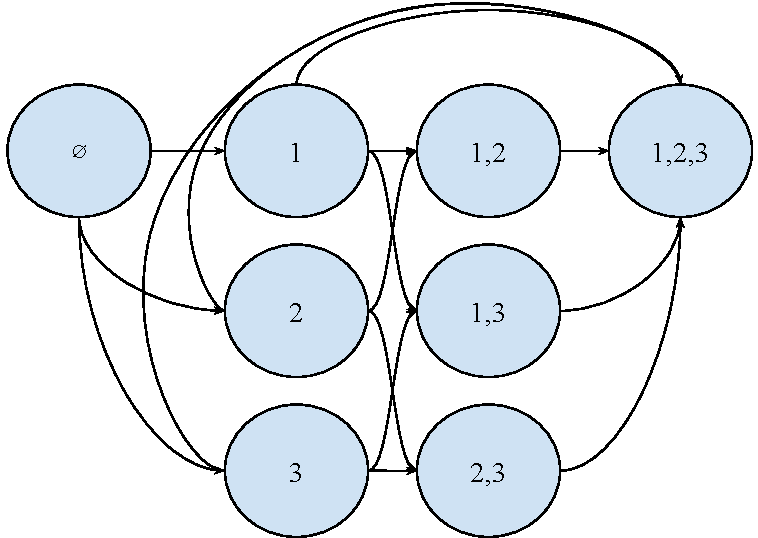
\includegraphics[width=0.75\linewidth]{MarkovStates.pdf}
\caption{Example of a Markov chain constructed for an election algorithm from information flows.}
\label{fig:markovstates}
\end{centering}
\end{figure}

\section{Election in an Anonymous Complete Network}

Consider a version of the "coin-flipping" leader election, expressed in terms of BIT logic.
This algorithm is functionally identical, but contains additional guards on the conditionals as an additional expression of the knowledge of the agents executing the algorithm.
Additionally, note that the construct of labeling each $\varphi$ that an agent receives is simply assigning labels to make the algorithm easier to reason about.
The algorithm only considers the complete collection of $\varphi$s for execution and not the source of any of the $\varphi$ used.

Additionally, let $\psi_i$ be the state where an agent completes the algorithm as the leader, and $\gamma_i$ is the state where an agent has terminated the algorithm.
Correct operation is where $\{\gamma_i : \forall i \}$ is true in the same round of execution and exactly one $\psi$ is true ($\sum_i \psi_i = 1$).

\begin{algorithm}
\caption{Anonymous Coin Flipping Leader Election Expressed in BIT logic}
\label{alg:coinflip}
\begin{algorithmic}[1]
\small
\State $\varphi_i \gets random(T,F)$
\State $\psi_i \gets F$
\State Send $\varphi_i$ to every active neighbor ($\forall j \neq i\ : I_j,i \varphi_i$)
\State Receive $\varphi_j$ from every active neighbor 
\If {$\varphi_i \wedge (\forall j \neq i, w \vDash V_{\varphi_j}^i(w) : \neg \varphi_j)$}
	\State $\psi_i \gets T$
	\State $\gamma_i \gets T$
\ElsIf {$(\varphi_i \wedge \exists j \neq i, w \vDash V_{\varphi_j}^i( \varphi_j)(w) : \varphi_j) \vee (\forall k$ s.t. $w \vDash V_{\varphi_k}^i(w) : \neg \varphi_k$}
	\State $\varphi_i \gets random(T,F)$
	\State Go to next round
\ElsIf {$\exists j \neq i, w \vDash V_{\varphi_j}^i(w) : \varphi_j$}
	\State $\gamma_i \gets T$
\EndIf
\end{algorithmic}
\end{algorithm}

\begin{thm}
Algorithm \ref{alg:coinflip} may not terminate correctly unless there is detectable, perfect information transfer to all parties in the algorithm.
\end{thm}

Proof: Let $i$ be the agent that would correctly terminate as the leader. Let $j$ be a process that has selected $\varphi_j = F$.

\begin{table}[h!]
\centering
\small
\begin{tabularx}{\linewidth}{l X X}
1. & $\varphi_i = T, \varphi_j = F$ & Initial conditions \\
2a.& $I_{j,i} \varphi_i$ & $i$ sends $\varphi_i$ to $j$ \\
2b.& $I_{i,j} \varphi_j$ & $j$ sends $\varphi_j$ to $i$ \\
3a.& $\neg (B_j I_{j,i} \varphi_i \wedge T_{j,i} \varphi_j)$ & $j$ does not receive $\varphi_i$. \\
3b.& $B_i I_{i,j} \varphi_j \wedge T_{i,j} \varphi_i$ & $i$ receives $\varphi_j$. \\
4a.& $\neg w \vDash V_{\varphi_i}{j}(w)$ & $j$ cannot valuate $\varphi_i$. \\
4b.& $B_i \varphi_j$ & By C1. \\
5a. & $\not \exists V_{\varphi_i}^j(w) \wedge \neg \varphi_j \rightarrow (\varphi \gets T)$ & $j$ Cannot determine that $i$ can terminate and incorrectly changes $\varphi$. \\
5b. & $\varphi_i \wedge w \vDash V_{\varphi_j}^i(w) \wedge \neg \varphi_j \rightarrow \psi_i$ & $i$ incorrectly terminates as the leader. \\

\end{tabularx} \\~\\
Therefore, $i$ will terminate before $j$ decides to go passive.
\label{tab:anonymityproof}
\end{table}

Which agrees with results from similar analysis CITE.
As with the Byzantine Generals problem, algorithms similar to Byzantine agreement can be constructed for the anonymous networks.
These algorithms terminate if the number of agents that omit information are less than a specific threshold. 
